% Options for packages loaded elsewhere
\PassOptionsToPackage{unicode}{hyperref}
\PassOptionsToPackage{hyphens}{url}
%
\documentclass[
  man, fleqn, noextraspace]{apa6}
\usepackage{lmodern}
\usepackage{amssymb,amsmath}
\usepackage{ifxetex,ifluatex}
\ifnum 0\ifxetex 1\fi\ifluatex 1\fi=0 % if pdftex
  \usepackage[T1]{fontenc}
  \usepackage[utf8]{inputenc}
  \usepackage{textcomp} % provide euro and other symbols
\else % if luatex or xetex
  \usepackage{unicode-math}
  \defaultfontfeatures{Scale=MatchLowercase}
  \defaultfontfeatures[\rmfamily]{Ligatures=TeX,Scale=1}
\fi
% Use upquote if available, for straight quotes in verbatim environments
\IfFileExists{upquote.sty}{\usepackage{upquote}}{}
\IfFileExists{microtype.sty}{% use microtype if available
  \usepackage[]{microtype}
  \UseMicrotypeSet[protrusion]{basicmath} % disable protrusion for tt fonts
}{}
\makeatletter
\@ifundefined{KOMAClassName}{% if non-KOMA class
  \IfFileExists{parskip.sty}{%
    \usepackage{parskip}
  }{% else
    \setlength{\parindent}{0pt}
    \setlength{\parskip}{6pt plus 2pt minus 1pt}}
}{% if KOMA class
  \KOMAoptions{parskip=half}}
\makeatother
\usepackage{xcolor}
\IfFileExists{xurl.sty}{\usepackage{xurl}}{} % add URL line breaks if available
\IfFileExists{bookmark.sty}{\usepackage{bookmark}}{\usepackage{hyperref}}
\hypersetup{
  pdftitle={Data Exploration of the 2005-2006 School Survey on Crime and Safety},
  pdfauthor={Jim Wright~\& Claire Zhang},
  pdfkeywords={School Crime, School Safety, Discipline Policies},
  hidelinks,
  pdfcreator={LaTeX via pandoc}}
\urlstyle{same} % disable monospaced font for URLs
\usepackage{graphicx,grffile}
\makeatletter
\def\maxwidth{\ifdim\Gin@nat@width>\linewidth\linewidth\else\Gin@nat@width\fi}
\def\maxheight{\ifdim\Gin@nat@height>\textheight\textheight\else\Gin@nat@height\fi}
\makeatother
% Scale images if necessary, so that they will not overflow the page
% margins by default, and it is still possible to overwrite the defaults
% using explicit options in \includegraphics[width, height, ...]{}
\setkeys{Gin}{width=\maxwidth,height=\maxheight,keepaspectratio}
% Set default figure placement to htbp
\makeatletter
\def\fps@figure{htbp}
\makeatother
\setlength{\emergencystretch}{3em} % prevent overfull lines
\providecommand{\tightlist}{%
  \setlength{\itemsep}{0pt}\setlength{\parskip}{0pt}}
\setcounter{secnumdepth}{-\maxdimen} % remove section numbering
\shorttitle{2005-2006 SCHOOL SURVEY ON CRIME AND SAFETY}
\affiliation{
\vspace{0.5cm}
\textsuperscript{1} University of Oregon}
\keywords{School Crime, School Safety, Discipline Policies\newline\indent Word count: 2,888}
\usepackage{csquotes}
\usepackage{upgreek}
\captionsetup{font=singlespacing,justification=justified}

\usepackage{longtable}
\usepackage{lscape}
\usepackage{multirow}
\usepackage{tabularx}
\usepackage[flushleft]{threeparttable}
\usepackage{threeparttablex}

\newenvironment{lltable}{\begin{landscape}\begin{center}\begin{ThreePartTable}}{\end{ThreePartTable}\end{center}\end{landscape}}

\makeatletter
\newcommand\LastLTentrywidth{1em}
\newlength\longtablewidth
\setlength{\longtablewidth}{1in}
\newcommand{\getlongtablewidth}{\begingroup \ifcsname LT@\roman{LT@tables}\endcsname \global\longtablewidth=0pt \renewcommand{\LT@entry}[2]{\global\advance\longtablewidth by ##2\relax\gdef\LastLTentrywidth{##2}}\@nameuse{LT@\roman{LT@tables}} \fi \endgroup}


\DeclareDelayedFloatFlavor{ThreePartTable}{table}
\DeclareDelayedFloatFlavor{lltable}{table}
\DeclareDelayedFloatFlavor*{longtable}{table}
\makeatletter
\renewcommand{\efloat@iwrite}[1]{\immediate\expandafter\protected@write\csname efloat@post#1\endcsname{}}
\makeatother
\raggedbottom
\setlength{\parskip}{0pt}

\title{Data Exploration of the 2005-2006 School Survey on Crime and Safety}
\author{Jim Wright\textsuperscript{1}~\& Claire Zhang\textsuperscript{1}}
\date{}

\authornote{This project was completed as part of a term assignment for EDLD 610: Intro to Data Science during the Fall 2019 term.

Correspondence concerning this article should be addressed to Jim Wright, University of Oregon, Eugene, OR. E-mail: \href{mailto:jwrigh16@uoregon.edu}{\nolinkurl{jwrigh16@uoregon.edu}}}

\abstract{
The purpose of this paper is to explore data from ``2005-2006 School Survey on Crime and Safety'' using functions in R Markdown. The data file with results from the survey was published by National Center for Education Statistics (NCES) and consists of 525 columns by 2,724 rows. We acquired it from data.gov website. To complete this project, 14 total variables were selected from the data set to transform from its messy state to tidy data. The 14 variables included the school ID variable, four categorical variables, five logical variables, and four quantitative variables. Linear models were completed to determine which categorical variables most highly correlated with total disciplinary actions within the school and to explore the possible correlation between the provision of teacher training and out of school suspensions (OSS). Results of the analyses found that the strongest predictors of disciplinary actions taken by schools are schools that were coded as either a high school or combined middle school and high school located in an urban city with a minority percentage of 20\% or more. It was also determined that the provision of teacher training occurred in a majority of schools; however, we didn't find these trainings have a significant impact on reducing the number of out of school suspensions.


}

\begin{document}
\maketitle

\hypertarget{introduction}{%
\section{Introduction}\label{introduction}}

Since the 1990s, there has been an increase in awareness and concern over the rate of school crime in American public schools (Chen, 2008). Following the 1999-2000 academic school year in which 71\% of American public schools experienced at least one violent incident, schools, predominantly in urban areas, responded with a variety of measures to curb violence. Such measures included the use of metal detectors, camera surveillance systems, and establishing a consistent police presence (Chen, 2008; Han \& Akiba, 2011). Schools have also placed more authority in the hands of classroom teachers to discipline students on an individual basis (Han \& Akiba, 2011).

The shift in school aggressiveness to prevent and discipline crime can be traced back to the 1994 Gun-Free Schools Act (GFSA), which was reauthorized in the 2001 No Child Left Behind Act (NCBL) (Han \& Akiba, 2011). There is a general consensus in the literature that more aggressive discipline policies authorized under GFSA and NCBL have not resulted in positive outcomes, but instead, have resulted in disproportionate discipline of students by certain characteristics such as student race, school size, school location, school level, school minority status, and school socioeconomic status (Han \& Akiba, 2011). Disproportionate discipline implementation may provide one rationale as to why specific student demographics, such as age, race, poverty, and socioeconomic status are highly correlated with school crime and violence.

Therefore, the purpose of this paper is to utilize functions within R Markdown to explore the results of the 2005-2006 School Survey on Crime and Safety with a specific focus on how school characteristics and the provision of specific types of teacher trainings correlate with total disciplinary actions.\\
\# Methods

The School Survey on Crime and Safety was first introduced during the 1999-2000 academic school year. It was repeated during the 2003-2004 school year and again in 2005-2006 (Nolle, Guerino, Dinkes, \& Chandler, 2007). The data to be explored and analyzed for this project represents the 2005-2006 school year, the third time the survey was distributed across U.S. public schools. Data collection for the survey began on March 17, 2006, and continued through May 26, 2006 (Nolle et al., 2007). The survey was sent to be completed by school principals of a stratified random sample of 3,565 schools. A total of 2,724 principals from primary, middle, high, and combined schools completed and returned the survey for a response rate of 81\% (Nolle et al., 2007).
\#\# Data Import

The survey data for this paper was obtained for free from data.gov. It was downloaded from the data.gov website as an SPSS file and imported into R for the purposes of data exploration and analysis. When imported into R, the data in its messy form consisted of 525 columns representing the questions of the survey and 2,724 rows representing the responses from each individual school.

The specific research questions for this paper were to explore how school characteristics and the provision of teacher training align with and predict school disciplinary actions. To address these questions, 14 variables, including the column identifying the specific school, were isolated from the complete data set using the \texttt{select()} function. These variables included four categorical variables, five logical variables, and four quantitative variables.

The four categorical variables were titled \enquote{urban}, \enquote{level}, \enquote{minority}, and \enquote{enroll} and each contained four levels. The \enquote{urban}, \enquote{minority}, and \enquote{enroll} variables were renamed in R Markdown using the \texttt{rename(}) function. The \enquote{urban} variable was renamed \enquote{urbanicity} to represent the variable of school urbanicity. Its four levels included: \emph{city}, \emph{urban fringe}, \emph{town}, and \emph{rural}. Although not renamed, the \enquote{level} variable represented the school's level and contained the following four levels: \emph{primary}, \emph{middle}, \emph{high school}, and \emph{combined}. Schools coded as \emph{combined} provided both middle and high school grades. The \enquote{minority} variable was renamed \enquote{minority status} to represent the variable of school minority status and contained the following four levels: \emph{less than 5 percent}, \emph{5 to 20 percent}, \emph{20 to 50 percent}, and \emph{greater than 50 percent}. The \enquote{enroll} variable was renamed \enquote{enrollment} and contained four levels to represent school enrollment. The four levels consisted of: \emph{less than 300}, \emph{300 - 499}, \emph{500 - 999}, and \emph{1,000 or more}.

The five logical variables of the organized data set represented logical variables with a yes/no response on whether or not the school provided specific types of teacher trainings. The five teacher trainings selected for the current project included: classroom management, discipline policies, safety procedures, early warning signs for violent behavior, and positive behavioral intervention. The variable names for teacher training were also renamed within R Markdown using the \texttt{rename()} function.

The four quantitative variables of the organized data set represented numerical counts of specific types of disciplinary actions taken by the school. The four types of disciplinary actions included: disciplinary actions recorded, incidents recorded, incidents reported to police, and out-of-school suspensions. Like the other variable types, the names of these variables were renamed using the \texttt{rename()} function in R Markdown. To make the analysis of these totals more efficient, these variables were combined into a single variable using the \texttt{mutate()} function to represent the total number of disciplinary actions per school.

\hypertarget{tidy-data}{%
\subsection{Tidy Data}\label{tidy-data}}

To tidy the data set aligning to our research questions, the \texttt{pivot\_longer()}, \texttt{pivot\_wider()}, and \texttt{filter()} functions were utilized. First, the average number of total disciplinary actions was identified and saved in R Markdown as its own object. Then, using pivot-longer() a new data frame was created in which the four disciplinary action variables were lengthened within the data set to more efficiently visualize the specific number of disciplinary actions (by type) per school. This new data frame only included schools with an above-average number of total disciplinary actions and that did not provide any type of teacher training. The schools for this data frame were identified using the filter() function. This data frame was then returned to its original form using the function pivot\_wider() to produce plots on the specific types of disciplinary actions. Plots for the tidy data frames are presented in Plots 1-5 and Tables 1 and 2.

\hypertarget{linear-models}{%
\subsection{Linear Models}\label{linear-models}}

To analyze the data by categorical variables as a predictor of total disciplinary actions, three linear models were constructed. The first model consisted of two categorical variables, school urbanicity and enrollment, to predict the total number of school disciplinary actions. The second and third models expanded upon the first model by adding an additional variable within each one. The second model added the variable of school level, and the third model added the variable of school minority status. The group\_by() and summarize() functions were then utilized to present each model in table form.

\hypertarget{descriptive-data-exploration-and-visualization}{%
\subsection{Descriptive Data Exploration and Visualization}\label{descriptive-data-exploration-and-visualization}}

The entire selected data set was utilized to produce Plots 6-10. These plots present different visualizations of the categorical variables, specifically the urbanicity variable. One scatterplot, Plot 8, was produced to display the relationship of out of school suspensions (OSS) to school total disciplinary actions.

\hypertarget{teacher-training-relationship-to-oss}{%
\subsection{Teacher Training Relationship to OSS}\label{teacher-training-relationship-to-oss}}

The final code chunk was produced in R Markdown to explore the relationship between the provision of teacher training and OSS. The pivot\_longer() function was utilized to identify and visualize the provision of the individual type of teacher training per school. Plot 11 displays the findings of this code.

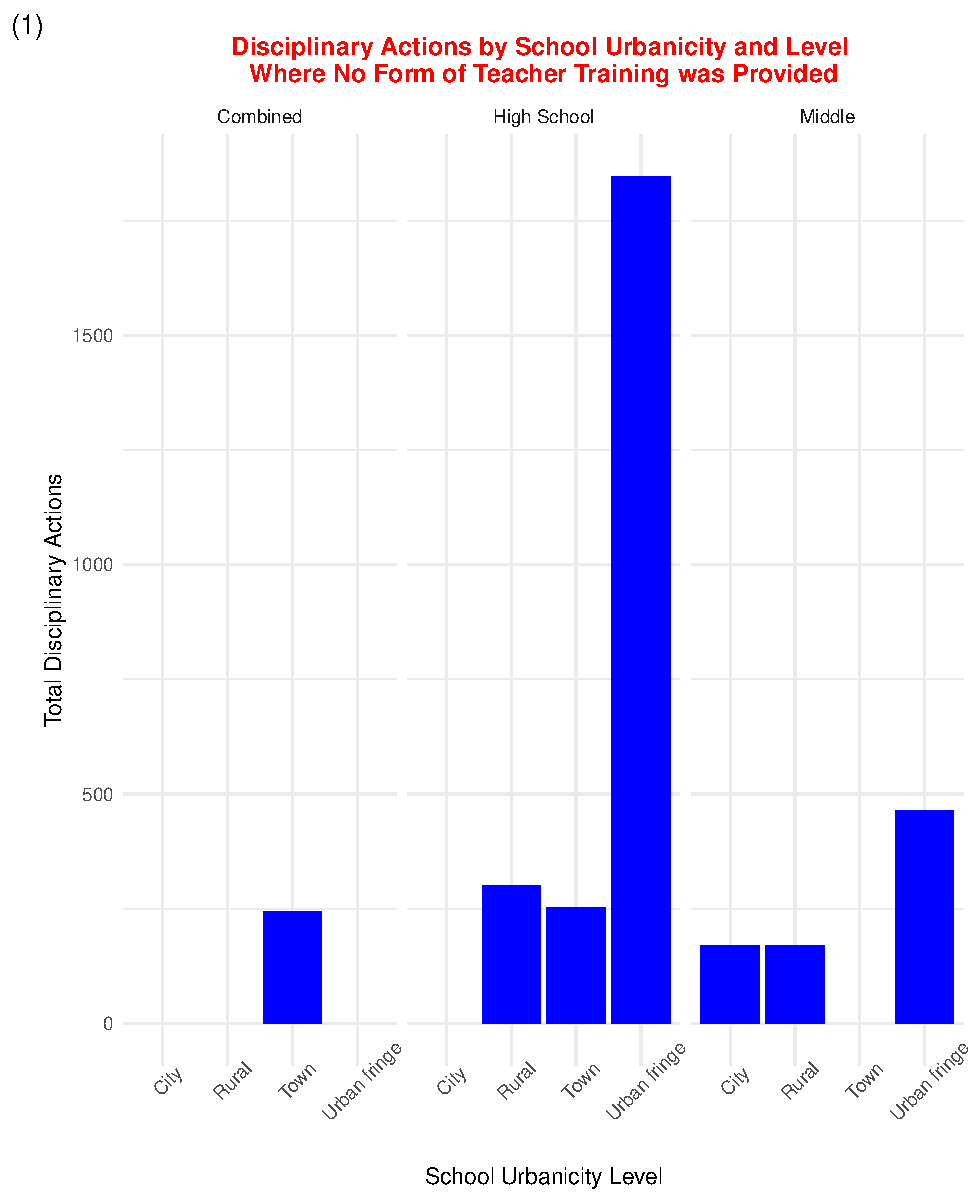
\includegraphics{Final-Project_Zhang_Wright_files/figure-latex/plots-tidydisc1-1.pdf} 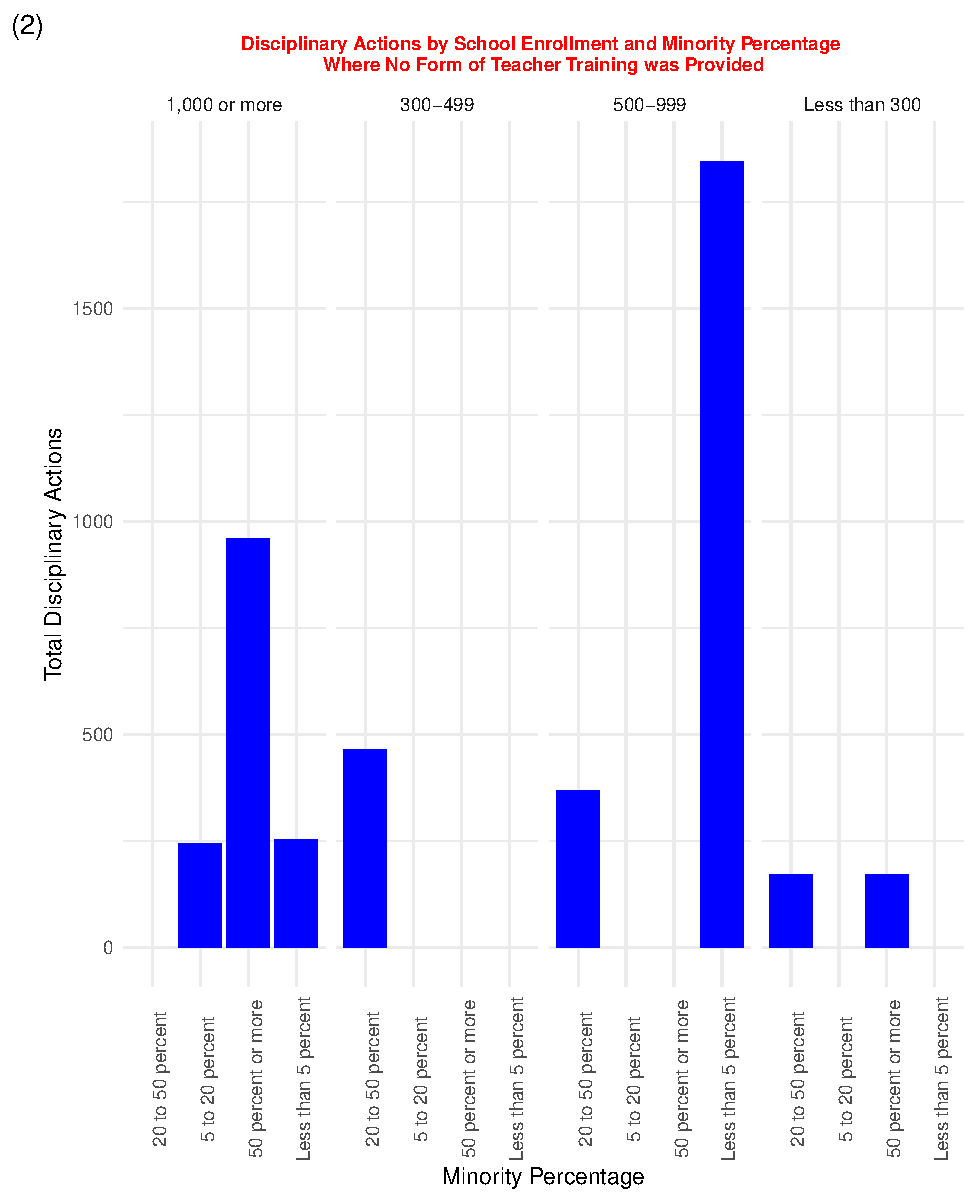
\includegraphics{Final-Project_Zhang_Wright_files/figure-latex/plots-tidydisc1-2.pdf} 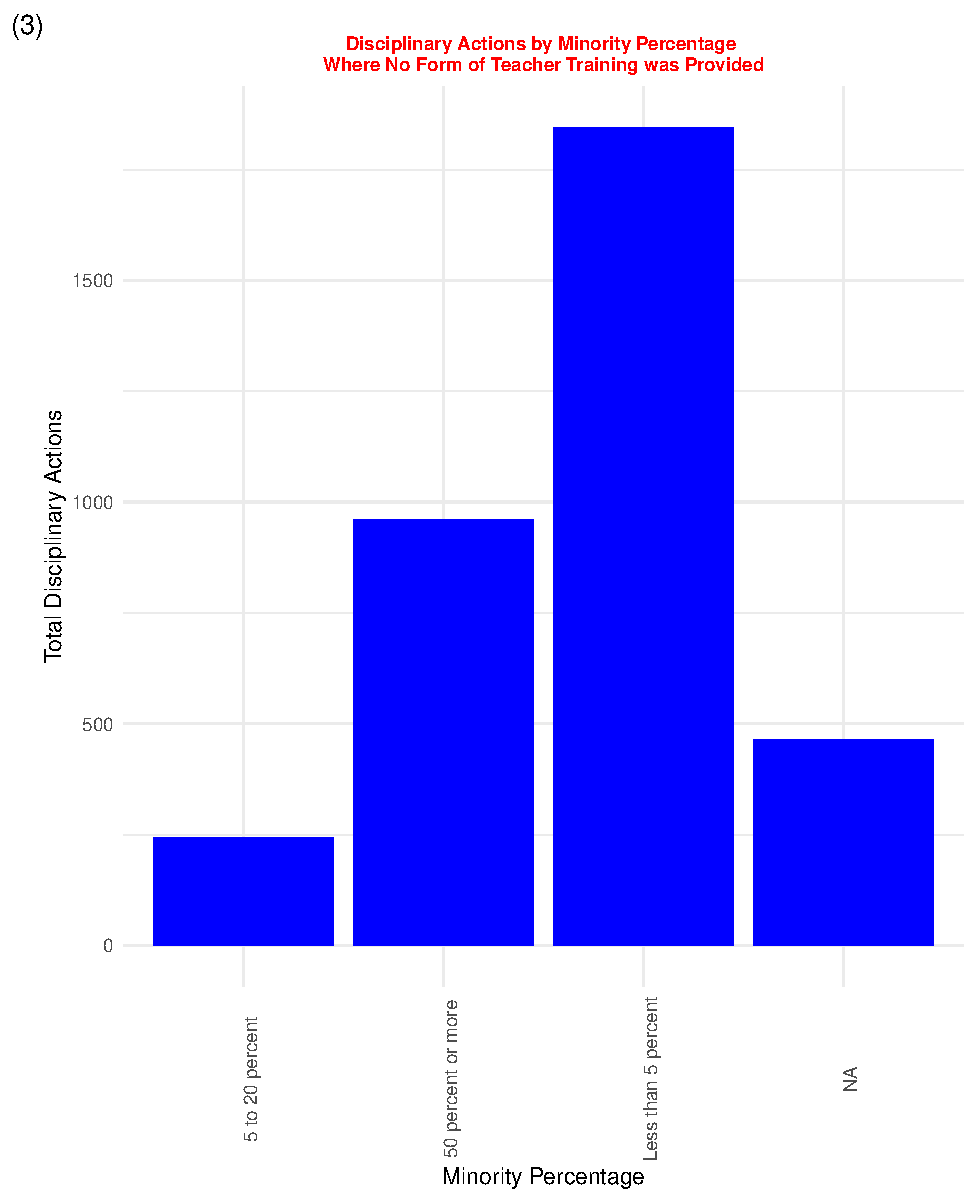
\includegraphics{Final-Project_Zhang_Wright_files/figure-latex/plots-tidydisc1-3.pdf}

\begin{table}[tbp]
\begin{center}
\begin{threeparttable}
\caption{\label{tab:descriptives tidydisc1}Total Disciplinary Actions for Schools Not Providing Any Form of Teacher Training by School Category}
\begin{tabular}{llllll}
\toprule
school\_id & \multicolumn{1}{c}{urbanicity} & \multicolumn{1}{c}{level} & \multicolumn{1}{c}{minority\_percentage} & \multicolumn{1}{c}{enrollment} & \multicolumn{1}{c}{sum(total\_discipline\_actions)}\\
\midrule
521.00 & Urban fringe & High School & 50 percent or more & 1,000 or more & 3,840.00\\
1,538.00 & Town & Combined & 5 to 20 percent & 1,000 or more & 972.00\\
1,802.00 & City & Middle & 50 percent or more & Less than 300 & 680.00\\
1,877.00 & Town & High School & Less than 5 percent & 1,000 or more & 1,012.00\\
2,823.00 & Rural & High School & 20 to 50 percent & 500-999 & 1,204.00\\
2,834.00 & Urban fringe & Middle & 20 to 50 percent & 500-999 & 1,476.00\\
2,879.00 & Urban fringe & High School & Less than 5 percent & 500-999 & 7,384.00\\
3,396.00 & Urban fringe & Middle & 5 to 20 percent & 1,000 or more & 828.00\\
3,397.00 & Urban fringe & Middle & 20 to 50 percent & 300-499 & 1,856.00\\
3,517.00 & Rural & Middle & 20 to 50 percent & Less than 300 & 680.00\\
\bottomrule
\end{tabular}
\end{threeparttable}
\end{center}
\end{table}

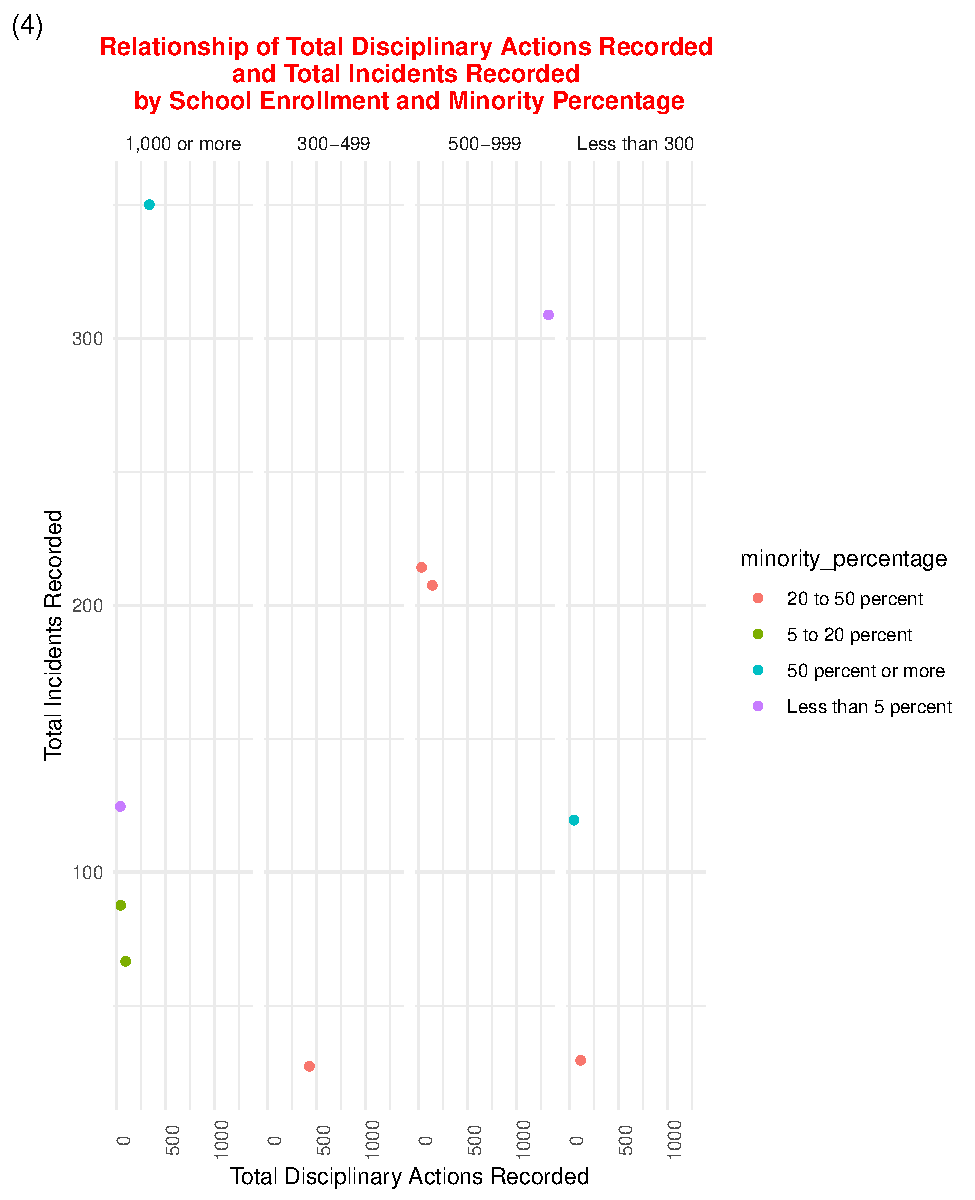
\includegraphics{Final-Project_Zhang_Wright_files/figure-latex/plots-tidydisc2-1.pdf} 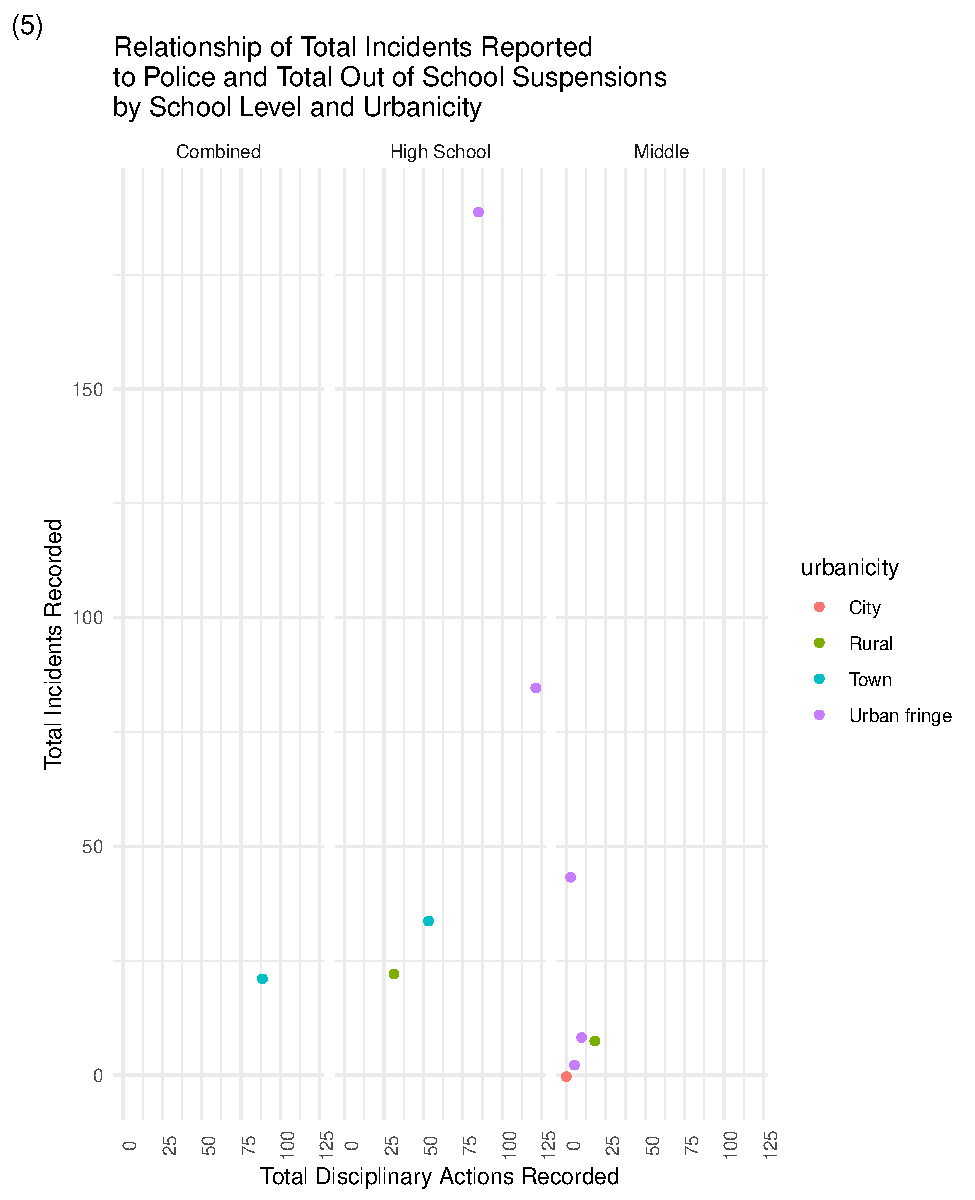
\includegraphics{Final-Project_Zhang_Wright_files/figure-latex/plots-tidydisc2-2.pdf}

\begin{table}[tbp]
\begin{center}
\begin{threeparttable}
\caption{\label{tab:descriptives tidydisc2}Total Disciplinary Actions for Schools Not Providing Any Form of Teacher Training by Specific Form of Discipline}
\begin{tabular}{llllll}
\toprule
school\_id & \multicolumn{1}{c}{total\_discipline\_actions} & \multicolumn{1}{c}{incidents\_recorded} & \multicolumn{1}{c}{incidents\_reported\_to\_police} & \multicolumn{1}{c}{out\_of\_school\_suspensions} & \multicolumn{1}{c}{sum(total\_discipline\_actions)}\\
\midrule
521.00 & 960.00 & 350.00 & 85.00 & 189.00 & 960.00\\
1,538.00 & 243.00 & 88.00 & 88.00 & 21.00 & 243.00\\
1,802.00 & 170.00 & 120.00 & 0.00 & 0.00 & 170.00\\
1,877.00 & 253.00 & 124.00 & 53.00 & 34.00 & 253.00\\
2,823.00 & 301.00 & 214.00 & 32.00 & 22.00 & 301.00\\
2,834.00 & 369.00 & 207.00 & 9.00 & 8.00 & 369.00\\
2,879.00 & 1,846.00 & 308.00 & 122.00 & 85.00 & 1,846.00\\
3,396.00 & 207.00 & 66.00 & 2.00 & 43.00 & 207.00\\
3,397.00 & 464.00 & 28.00 & 5.00 & 2.00 & 464.00\\
3,517.00 & 170.00 & 30.00 & 18.00 & 7.00 & 170.00\\
\bottomrule
\end{tabular}
\end{threeparttable}
\end{center}
\end{table}

\begin{table}[tbp]
\begin{center}
\begin{threeparttable}
\caption{\label{tab:model tables}Regression Results displaying Total Disciplinary Actions Predicted by School Urbanicity when Controlling for School Enrollment}
\begin{tabular}{lll}
\toprule
urbanicity & \multicolumn{1}{c}{enrollment} & \multicolumn{1}{c}{total\_discipline\_actions}\\
\midrule
City & 1,000 or more & 103,504.00\\
City & 300-499 & 8,964.00\\
City & 500-999 & 37,112.00\\
City & Less than 300 & 2,673.00\\
Rural & 1,000 or more & 21,629.00\\
Rural & 300-499 & 9,817.00\\
Rural & 500-999 & 26,981.00\\
Rural & Less than 300 & 7,802.00\\
Town & 1,000 or more & 11,441.00\\
Town & 300-499 & 5,190.00\\
Town & 500-999 & 15,869.00\\
Town & Less than 300 & 1,354.00\\
Urban fringe & 1,000 or more & 112,389.00\\
Urban fringe & 300-499 & 10,233.00\\
Urban fringe & 500-999 & 54,830.00\\
Urban fringe & Less than 300 & 2,742.00\\
\bottomrule
\end{tabular}
\end{threeparttable}
\end{center}
\end{table}

\begin{table}[tbp]
\begin{center}
\begin{threeparttable}
\caption{\label{tab:model tables}Regression Results displaying Total Disciplinary Actions Predicted by School Urbanicity when Controlling for School Enrollment and Level}
\begin{tabular}{llll}
\toprule
urbanicity & \multicolumn{1}{c}{enrollment} & \multicolumn{1}{c}{level} & \multicolumn{1}{c}{total\_discipline\_actions}\\
\midrule
City & 1,000 or more & Combined & 1,989.00\\
City & 1,000 or more & High School & 77,226.00\\
City & 1,000 or more & Middle & 23,203.00\\
City & 1,000 or more & Primary & 1,086.00\\
City & 300-499 & Combined & 147.00\\
City & 300-499 & High School & 98.00\\
City & 300-499 & Middle & 4,894.00\\
City & 300-499 & Primary & 3,825.00\\
City & 500-999 & Combined & 556.00\\
City & 500-999 & High School & 3,694.00\\
City & 500-999 & Middle & 25,519.00\\
City & 500-999 & Primary & 7,343.00\\
City & Less than 300 & Combined & 73.00\\
City & Less than 300 & High School & 321.00\\
City & Less than 300 & Middle & 1,402.00\\
City & Less than 300 & Primary & 877.00\\
Rural & 1,000 or more & Combined & 158.00\\
Rural & 1,000 or more & High School & 19,052.00\\
Rural & 1,000 or more & Middle & 2,412.00\\
Rural & 1,000 or more & Primary & 7.00\\
Rural & 300-499 & Combined & 1,367.00\\
Rural & 300-499 & High School & 3,180.00\\
Rural & 300-499 & Middle & 4,128.00\\
Rural & 300-499 & Primary & 1,142.00\\
Rural & 500-999 & Combined & 1,762.00\\
Rural & 500-999 & High School & 12,210.00\\
Rural & 500-999 & Middle & 11,221.00\\
Rural & 500-999 & Primary & 1,788.00\\
Rural & Less than 300 & Combined & 1,103.00\\
Rural & Less than 300 & High School & 2,774.00\\
Rural & Less than 300 & Middle & 3,076.00\\
Rural & Less than 300 & Primary & 849.00\\
Town & 1,000 or more & Combined & 771.00\\
Town & 1,000 or more & High School & 8,546.00\\
Town & 1,000 or more & Middle & 2,111.00\\
Town & 1,000 or more & Primary & 13.00\\
Town & 300-499 & Combined & 128.00\\
Town & 300-499 & High School & 1,731.00\\
Town & 300-499 & Middle & 2,878.00\\
Town & 300-499 & Primary & 453.00\\
Town & 500-999 & Combined & 247.00\\
Town & 500-999 & High School & 5,520.00\\
Town & 500-999 & Middle & 9,119.00\\
Town & 500-999 & Primary & 983.00\\
Town & Less than 300 & Combined & 123.00\\
Town & Less than 300 & High School & 323.00\\
Town & Less than 300 & Middle & 589.00\\
Town & Less than 300 & Primary & 319.00\\
Urban fringe & 1,000 or more & Combined & 1,274.00\\
Urban fringe & 1,000 or more & High School & 81,214.00\\
Urban fringe & 1,000 or more & Middle & 29,046.00\\
Urban fringe & 1,000 or more & Primary & 855.00\\
Urban fringe & 300-499 & Combined & 24.00\\
Urban fringe & 300-499 & High School & 1,385.00\\
Urban fringe & 300-499 & Middle & 6,054.00\\
Urban fringe & 300-499 & Primary & 2,770.00\\
Urban fringe & 500-999 & Combined & 299.00\\
Urban fringe & 500-999 & High School & 12,041.00\\
Urban fringe & 500-999 & Middle & 36,841.00\\
Urban fringe & 500-999 & Primary & 5,649.00\\
Urban fringe & Less than 300 & Combined & 128.00\\
Urban fringe & Less than 300 & High School & 599.00\\
Urban fringe & Less than 300 & Middle & 1,713.00\\
Urban fringe & Less than 300 & Primary & 302.00\\
\bottomrule
\end{tabular}
\end{threeparttable}
\end{center}
\end{table}

\begin{table}[tbp]
\begin{center}
\begin{threeparttable}
\caption{\label{tab:model tables}Regression Results displaying Total Disciplinary Actions Predicted by School Urbanicity when Controlling for School Enrollment, Level, and Minority Percentage}
\begin{tabular}{lllll}
\toprule
urbanicity & \multicolumn{1}{c}{enrollment} & \multicolumn{1}{c}{level} & \multicolumn{1}{c}{minority\_percentage} & \multicolumn{1}{c}{total\_discipline\_actions}\\
\midrule
City & 1,000 or more & Combined & 20 to 50 percent & 667.00\\
City & 1,000 or more & Combined & 5 to 20 percent & 455.00\\
City & 1,000 or more & Combined & 50 percent or more & 492.00\\
City & 1,000 or more & High School & 20 to 50 percent & 24,003.00\\
City & 1,000 or more & High School & 5 to 20 percent & 9,466.00\\
City & 1,000 or more & High School & 50 percent or more & 41,835.00\\
City & 1,000 or more & High School & Less than 5 percent & 119.00\\
City & 1,000 or more & Middle & 20 to 50 percent & 7,009.00\\
City & 1,000 or more & Middle & 5 to 20 percent & 657.00\\
City & 1,000 or more & Middle & 50 percent or more & 13,239.00\\
City & 1,000 or more & Primary & 20 to 50 percent & 22.00\\
City & 1,000 or more & Primary & 50 percent or more & 1,064.00\\
City & 300-499 & Combined & 20 to 50 percent & 14.00\\
City & 300-499 & Combined & 50 percent or more & 21.00\\
City & 300-499 & High School & 20 to 50 percent & 12.00\\
City & 300-499 & High School & 5 to 20 percent & 20.00\\
City & 300-499 & High School & 50 percent or more & 66.00\\
City & 300-499 & Middle & 20 to 50 percent & 560.00\\
City & 300-499 & Middle & 5 to 20 percent & 559.00\\
City & 300-499 & Middle & 50 percent or more & 3,736.00\\
City & 300-499 & Primary & 20 to 50 percent & 801.00\\
City & 300-499 & Primary & 5 to 20 percent & 184.00\\
City & 300-499 & Primary & 50 percent or more & 2,832.00\\
City & 300-499 & Primary & Less than 5 percent & 8.00\\
City & 500-999 & Combined & 5 to 20 percent & 2.00\\
City & 500-999 & Combined & 50 percent or more & 554.00\\
City & 500-999 & High School & 20 to 50 percent & 142.00\\
City & 500-999 & High School & 5 to 20 percent & 417.00\\
City & 500-999 & High School & 50 percent or more & 3,016.00\\
City & 500-999 & Middle & 20 to 50 percent & 5,814.00\\
City & 500-999 & Middle & 5 to 20 percent & 2,664.00\\
City & 500-999 & Middle & 50 percent or more & 16,417.00\\
City & 500-999 & Primary & 20 to 50 percent & 573.00\\
City & 500-999 & Primary & 5 to 20 percent & 276.00\\
City & 500-999 & Primary & 50 percent or more & 6,287.00\\
City & 500-999 & Primary & Less than 5 percent & 54.00\\
City & Less than 300 & Combined & 20 to 50 percent & 35.00\\
City & Less than 300 & Combined & 50 percent or more & 38.00\\
City & Less than 300 & High School & 20 to 50 percent & 47.00\\
City & Less than 300 & High School & 5 to 20 percent & 40.00\\
City & Less than 300 & High School & 50 percent or more & 234.00\\
City & Less than 300 & Middle & 20 to 50 percent & 40.00\\
City & Less than 300 & Middle & 5 to 20 percent & 11.00\\
City & Less than 300 & Middle & 50 percent or more & 1,351.00\\
City & Less than 300 & Primary & 20 to 50 percent & 283.00\\
City & Less than 300 & Primary & 5 to 20 percent & 167.00\\
City & Less than 300 & Primary & 50 percent or more & 393.00\\
City & Less than 300 & Primary & Less than 5 percent & 27.00\\
Rural & 1,000 or more & Combined & 20 to 50 percent & 22.00\\
Rural & 1,000 or more & Combined & Less than 5 percent & 136.00\\
Rural & 1,000 or more & High School & 20 to 50 percent & 3,636.00\\
Rural & 1,000 or more & High School & 5 to 20 percent & 6,395.00\\
Rural & 1,000 or more & High School & 50 percent or more & 5,440.00\\
Rural & 1,000 or more & High School & Less than 5 percent & 3,124.00\\
Rural & 1,000 or more & Middle & 20 to 50 percent & 867.00\\
Rural & 1,000 or more & Middle & 5 to 20 percent & 1,062.00\\
Rural & 1,000 or more & Middle & 50 percent or more & 365.00\\
Rural & 1,000 or more & Middle & Less than 5 percent & 118.00\\
Rural & 1,000 or more & Primary & 20 to 50 percent & 7.00\\
Rural & 300-499 & Combined & 20 to 50 percent & 366.00\\
Rural & 300-499 & Combined & 5 to 20 percent & 316.00\\
Rural & 300-499 & Combined & 50 percent or more & 136.00\\
Rural & 300-499 & Combined & Less than 5 percent & 410.00\\
Rural & 300-499 & High School & 20 to 50 percent & 706.00\\
Rural & 300-499 & High School & 5 to 20 percent & 1,029.00\\
Rural & 300-499 & High School & 50 percent or more & 161.00\\
Rural & 300-499 & High School & Less than 5 percent & 1,155.00\\
Rural & 300-499 & Middle & 20 to 50 percent & 809.00\\
Rural & 300-499 & Middle & 5 to 20 percent & 419.00\\
Rural & 300-499 & Middle & 50 percent or more & 884.00\\
Rural & 300-499 & Middle & Less than 5 percent & 1,943.00\\
Rural & 300-499 & Primary & 20 to 50 percent & 243.00\\
Rural & 300-499 & Primary & 5 to 20 percent & 188.00\\
Rural & 300-499 & Primary & 50 percent or more & 291.00\\
Rural & 300-499 & Primary & Less than 5 percent & 333.00\\
Rural & 500-999 & Combined & 20 to 50 percent & 264.00\\
Rural & 500-999 & Combined & 5 to 20 percent & 419.00\\
Rural & 500-999 & Combined & 50 percent or more & 236.00\\
Rural & 500-999 & Combined & Less than 5 percent & 798.00\\
Rural & 500-999 & High School & 20 to 50 percent & 2,191.00\\
Rural & 500-999 & High School & 5 to 20 percent & 3,594.00\\
Rural & 500-999 & High School & 50 percent or more & 1,124.00\\
Rural & 500-999 & High School & Less than 5 percent & 4,545.00\\
Rural & 500-999 & Middle & 20 to 50 percent & 3,467.00\\
Rural & 500-999 & Middle & 5 to 20 percent & 2,259.00\\
Rural & 500-999 & Middle & 50 percent or more & 2,109.00\\
Rural & 500-999 & Middle & Less than 5 percent & 2,658.00\\
Rural & 500-999 & Primary & 20 to 50 percent & 258.00\\
Rural & 500-999 & Primary & 5 to 20 percent & 354.00\\
Rural & 500-999 & Primary & 50 percent or more & 718.00\\
Rural & 500-999 & Primary & Less than 5 percent & 443.00\\
Rural & Less than 300 & Combined & 20 to 50 percent & 233.00\\
Rural & Less than 300 & Combined & 5 to 20 percent & 250.00\\
Rural & Less than 300 & Combined & 50 percent or more & 143.00\\
Rural & Less than 300 & Combined & Less than 5 percent & 477.00\\
Rural & Less than 300 & High School & 20 to 50 percent & 424.00\\
Rural & Less than 300 & High School & 5 to 20 percent & 299.00\\
Rural & Less than 300 & High School & 50 percent or more & 631.00\\
Rural & Less than 300 & High School & Less than 5 percent & 1,420.00\\
Rural & Less than 300 & Middle & 20 to 50 percent & 700.00\\
Rural & Less than 300 & Middle & 5 to 20 percent & 710.00\\
Rural & Less than 300 & Middle & 50 percent or more & 348.00\\
Rural & Less than 300 & Middle & Less than 5 percent & 1,318.00\\
Rural & Less than 300 & Primary & 20 to 50 percent & 51.00\\
Rural & Less than 300 & Primary & 5 to 20 percent & 111.00\\
Rural & Less than 300 & Primary & 50 percent or more & 71.00\\
Rural & Less than 300 & Primary & Less than 5 percent & 590.00\\
Town & 1,000 or more & Combined & 5 to 20 percent & 243.00\\
Town & 1,000 or more & Combined & Less than 5 percent & 528.00\\
Town & 1,000 or more & High School & 20 to 50 percent & 2,230.00\\
Town & 1,000 or more & High School & 5 to 20 percent & 2,725.00\\
Town & 1,000 or more & High School & 50 percent or more & 1,299.00\\
Town & 1,000 or more & High School & Less than 5 percent & 1,500.00\\
Town & 1,000 or more & Middle & 20 to 50 percent & 868.00\\
Town & 1,000 or more & Middle & 5 to 20 percent & 635.00\\
Town & 1,000 or more & Middle & 50 percent or more & 608.00\\
Town & 1,000 or more & Primary & 5 to 20 percent & 13.00\\
Town & 300-499 & Combined & 20 to 50 percent & 110.00\\
Town & 300-499 & Combined & Less than 5 percent & 18.00\\
Town & 300-499 & High School & 20 to 50 percent & 251.00\\
Town & 300-499 & High School & 5 to 20 percent & 547.00\\
Town & 300-499 & High School & 50 percent or more & 521.00\\
Town & 300-499 & High School & Less than 5 percent & 412.00\\
Town & 300-499 & Middle & 20 to 50 percent & 757.00\\
Town & 300-499 & Middle & 5 to 20 percent & 629.00\\
Town & 300-499 & Middle & 50 percent or more & 836.00\\
Town & 300-499 & Middle & Less than 5 percent & 605.00\\
Town & 300-499 & Primary & 20 to 50 percent & 186.00\\
Town & 300-499 & Primary & 5 to 20 percent & 63.00\\
Town & 300-499 & Primary & 50 percent or more & 82.00\\
Town & 300-499 & Primary & Less than 5 percent & 95.00\\
Town & 500-999 & Combined & 5 to 20 percent & 32.00\\
Town & 500-999 & Combined & Less than 5 percent & 91.00\\
Town & 500-999 & High School & 20 to 50 percent & 1,379.00\\
Town & 500-999 & High School & 5 to 20 percent & 1,468.00\\
Town & 500-999 & High School & 50 percent or more & 1,268.00\\
Town & 500-999 & High School & Less than 5 percent & 1,269.00\\
Town & 500-999 & Middle & 20 to 50 percent & 1,885.00\\
Town & 500-999 & Middle & 5 to 20 percent & 1,680.00\\
Town & 500-999 & Middle & 50 percent or more & 4,142.00\\
Town & 500-999 & Middle & Less than 5 percent & 1,355.00\\
Town & 500-999 & Primary & 20 to 50 percent & 128.00\\
Town & 500-999 & Primary & 5 to 20 percent & 59.00\\
Town & 500-999 & Primary & 50 percent or more & 405.00\\
Town & 500-999 & Primary & Less than 5 percent & 391.00\\
Town & Less than 300 & Combined & 20 to 50 percent & 123.00\\
Town & Less than 300 & High School & 20 to 50 percent & 25.00\\
Town & Less than 300 & High School & 5 to 20 percent & 120.00\\
Town & Less than 300 & High School & 50 percent or more & 123.00\\
Town & Less than 300 & High School & Less than 5 percent & 55.00\\
Town & Less than 300 & Middle & 20 to 50 percent & 99.00\\
Town & Less than 300 & Middle & 5 to 20 percent & 76.00\\
Town & Less than 300 & Middle & 50 percent or more & 190.00\\
Town & Less than 300 & Middle & Less than 5 percent & 224.00\\
Town & Less than 300 & Primary & 20 to 50 percent & 52.00\\
Town & Less than 300 & Primary & 5 to 20 percent & 102.00\\
Town & Less than 300 & Primary & 50 percent or more & 55.00\\
Town & Less than 300 & Primary & Less than 5 percent & 110.00\\
Urban fringe & 1,000 or more & Combined & 20 to 50 percent & 152.00\\
Urban fringe & 1,000 or more & Combined & 5 to 20 percent & 401.00\\
Urban fringe & 1,000 or more & Combined & 50 percent or more & 308.00\\
Urban fringe & 1,000 or more & Combined & Less than 5 percent & 413.00\\
Urban fringe & 1,000 or more & High School & 20 to 50 percent & 24,226.00\\
Urban fringe & 1,000 or more & High School & 5 to 20 percent & 24,735.00\\
Urban fringe & 1,000 or more & High School & 50 percent or more & 25,739.00\\
Urban fringe & 1,000 or more & High School & Less than 5 percent & 4,823.00\\
Urban fringe & 1,000 or more & Middle & 20 to 50 percent & 9,133.00\\
Urban fringe & 1,000 or more & Middle & 5 to 20 percent & 6,200.00\\
Urban fringe & 1,000 or more & Middle & 50 percent or more & 13,160.00\\
Urban fringe & 1,000 or more & Middle & Less than 5 percent & 553.00\\
Urban fringe & 1,000 or more & Primary & 20 to 50 percent & 137.00\\
Urban fringe & 1,000 or more & Primary & 5 to 20 percent & 57.00\\
Urban fringe & 1,000 or more & Primary & 50 percent or more & 661.00\\
Urban fringe & 300-499 & Combined & 5 to 20 percent & 18.00\\
Urban fringe & 300-499 & Combined & 50 percent or more & 6.00\\
Urban fringe & 300-499 & High School & 20 to 50 percent & 703.00\\
Urban fringe & 300-499 & High School & 5 to 20 percent & 352.00\\
Urban fringe & 300-499 & High School & 50 percent or more & 222.00\\
Urban fringe & 300-499 & High School & Less than 5 percent & 108.00\\
Urban fringe & 300-499 & Middle & 20 to 50 percent & 1,090.00\\
Urban fringe & 300-499 & Middle & 5 to 20 percent & 3,033.00\\
Urban fringe & 300-499 & Middle & 50 percent or more & 1,146.00\\
Urban fringe & 300-499 & Middle & Less than 5 percent & 719.00\\
Urban fringe & 300-499 & Primary & 20 to 50 percent & 915.00\\
Urban fringe & 300-499 & Primary & 5 to 20 percent & 676.00\\
Urban fringe & 300-499 & Primary & 50 percent or more & 812.00\\
Urban fringe & 300-499 & Primary & Less than 5 percent & 345.00\\
Urban fringe & 500-999 & Combined & 20 to 50 percent & 225.00\\
Urban fringe & 500-999 & Combined & 5 to 20 percent & 39.00\\
Urban fringe & 500-999 & Combined & 50 percent or more & 35.00\\
Urban fringe & 500-999 & High School & 20 to 50 percent & 2,007.00\\
Urban fringe & 500-999 & High School & 5 to 20 percent & 4,532.00\\
Urban fringe & 500-999 & High School & 50 percent or more & 1,217.00\\
Urban fringe & 500-999 & High School & Less than 5 percent & 3,963.00\\
Urban fringe & 500-999 & Middle & 20 to 50 percent & 10,548.00\\
Urban fringe & 500-999 & Middle & 5 to 20 percent & 8,574.00\\
Urban fringe & 500-999 & Middle & 50 percent or more & 14,872.00\\
Urban fringe & 500-999 & Middle & Less than 5 percent & 1,465.00\\
Urban fringe & 500-999 & Primary & 20 to 50 percent & 1,079.00\\
Urban fringe & 500-999 & Primary & 5 to 20 percent & 1,425.00\\
Urban fringe & 500-999 & Primary & 50 percent or more & 2,948.00\\
Urban fringe & 500-999 & Primary & Less than 5 percent & 129.00\\
Urban fringe & Less than 300 & Combined & 20 to 50 percent & 96.00\\
Urban fringe & Less than 300 & Combined & 5 to 20 percent & 14.00\\
Urban fringe & Less than 300 & Combined & Less than 5 percent & 18.00\\
Urban fringe & Less than 300 & High School & 20 to 50 percent & 113.00\\
Urban fringe & Less than 300 & High School & 5 to 20 percent & 183.00\\
Urban fringe & Less than 300 & High School & 50 percent or more & 168.00\\
Urban fringe & Less than 300 & High School & Less than 5 percent & 135.00\\
Urban fringe & Less than 300 & Middle & 20 to 50 percent & 396.00\\
Urban fringe & Less than 300 & Middle & 5 to 20 percent & 394.00\\
Urban fringe & Less than 300 & Middle & 50 percent or more & 240.00\\
Urban fringe & Less than 300 & Middle & Less than 5 percent & 683.00\\
Urban fringe & Less than 300 & Primary & 20 to 50 percent & 96.00\\
Urban fringe & Less than 300 & Primary & 5 to 20 percent & 43.00\\
Urban fringe & Less than 300 & Primary & 50 percent or more & 113.00\\
Urban fringe & Less than 300 & Primary & Less than 5 percent & 50.00\\
\bottomrule
\end{tabular}
\end{threeparttable}
\end{center}
\end{table}

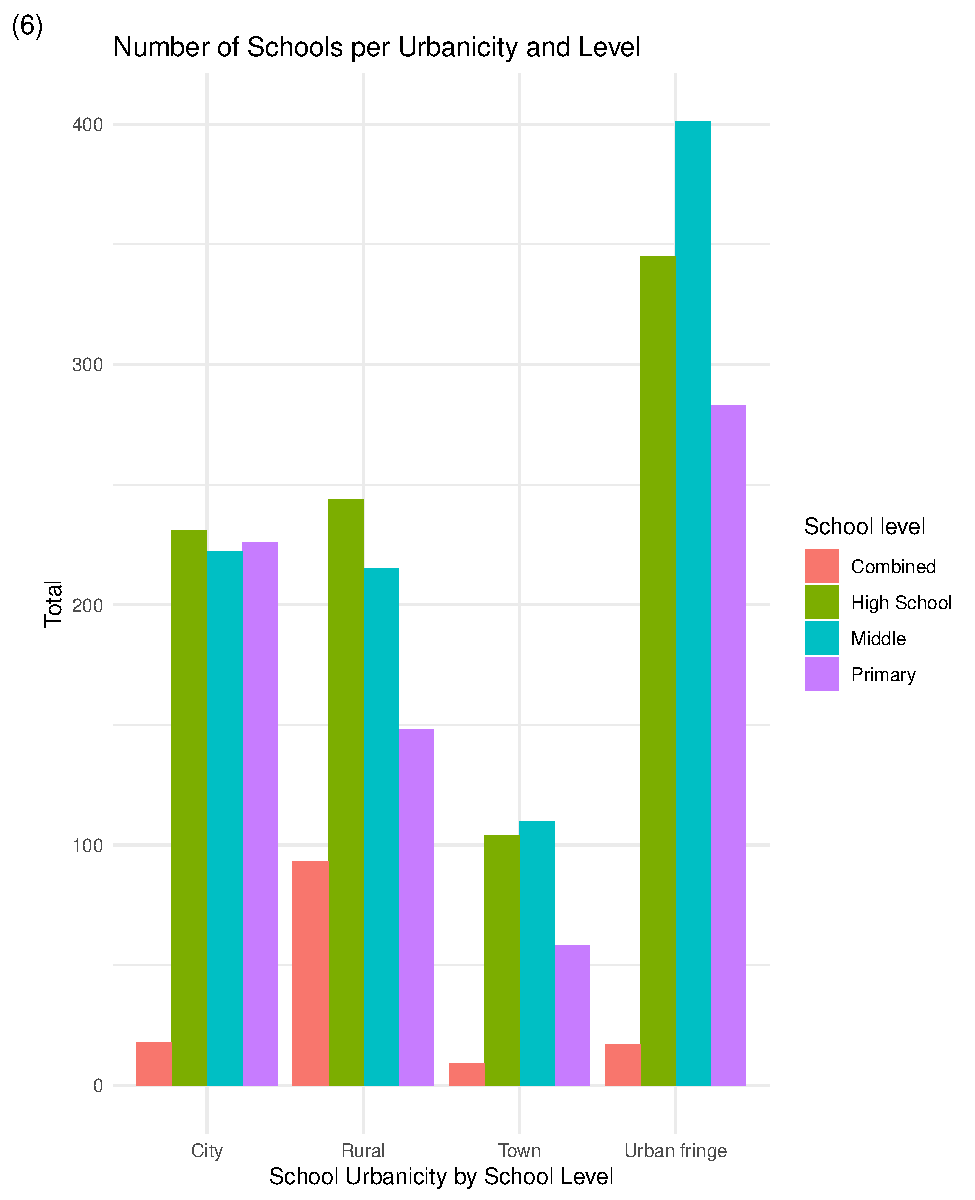
\includegraphics{Final-Project_Zhang_Wright_files/figure-latex/descriptives all selected data-1.pdf} 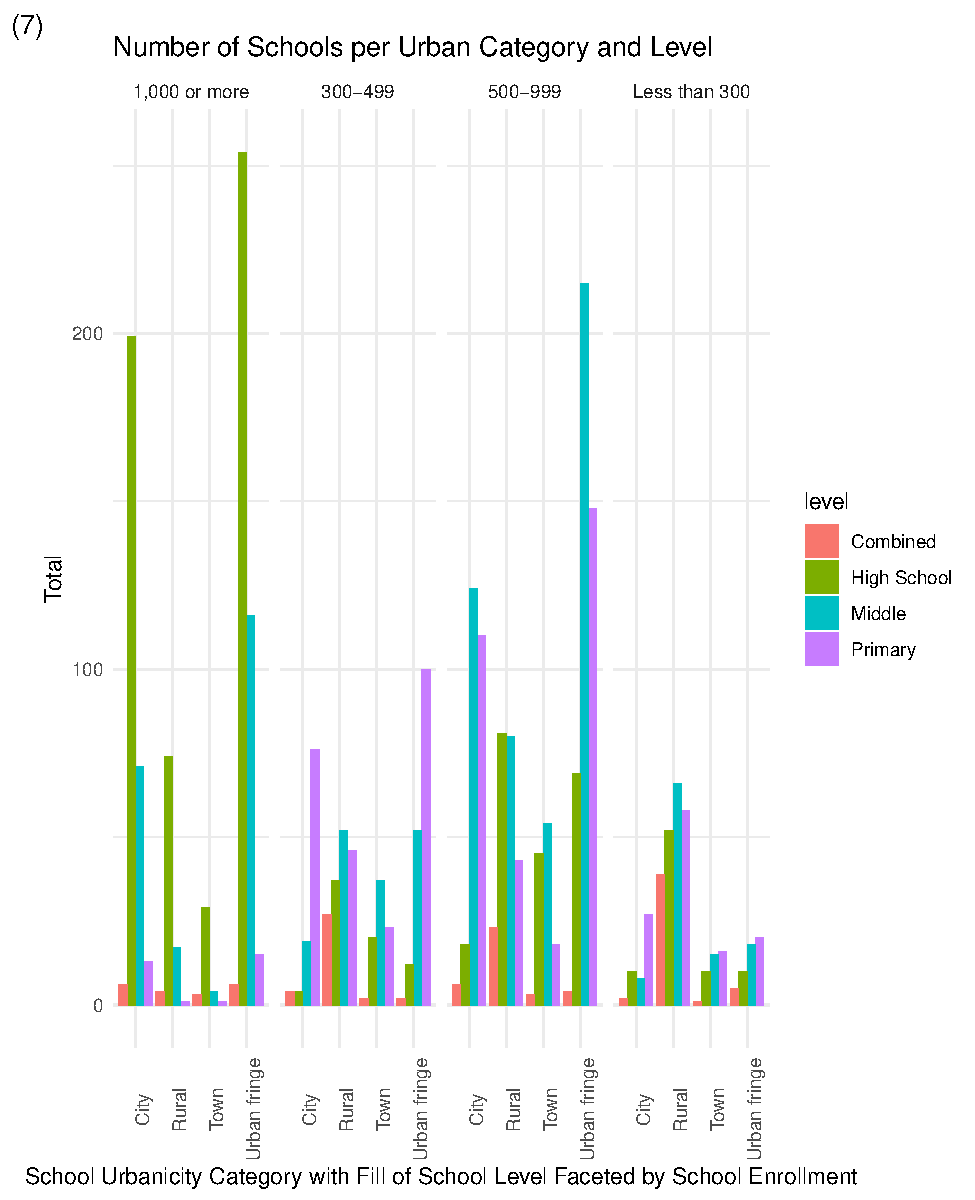
\includegraphics{Final-Project_Zhang_Wright_files/figure-latex/descriptives all selected data-2.pdf} 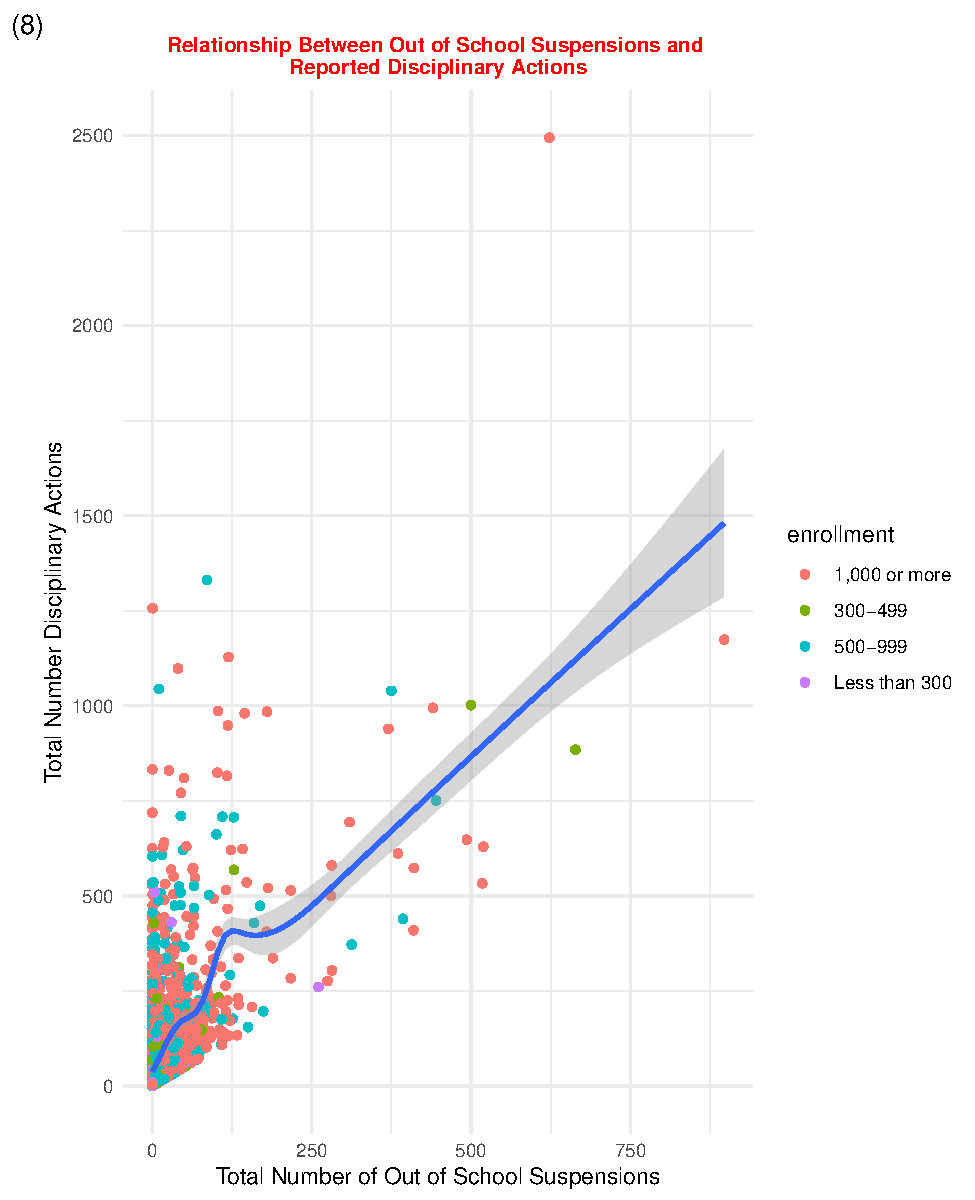
\includegraphics{Final-Project_Zhang_Wright_files/figure-latex/descriptives all selected data-3.pdf} 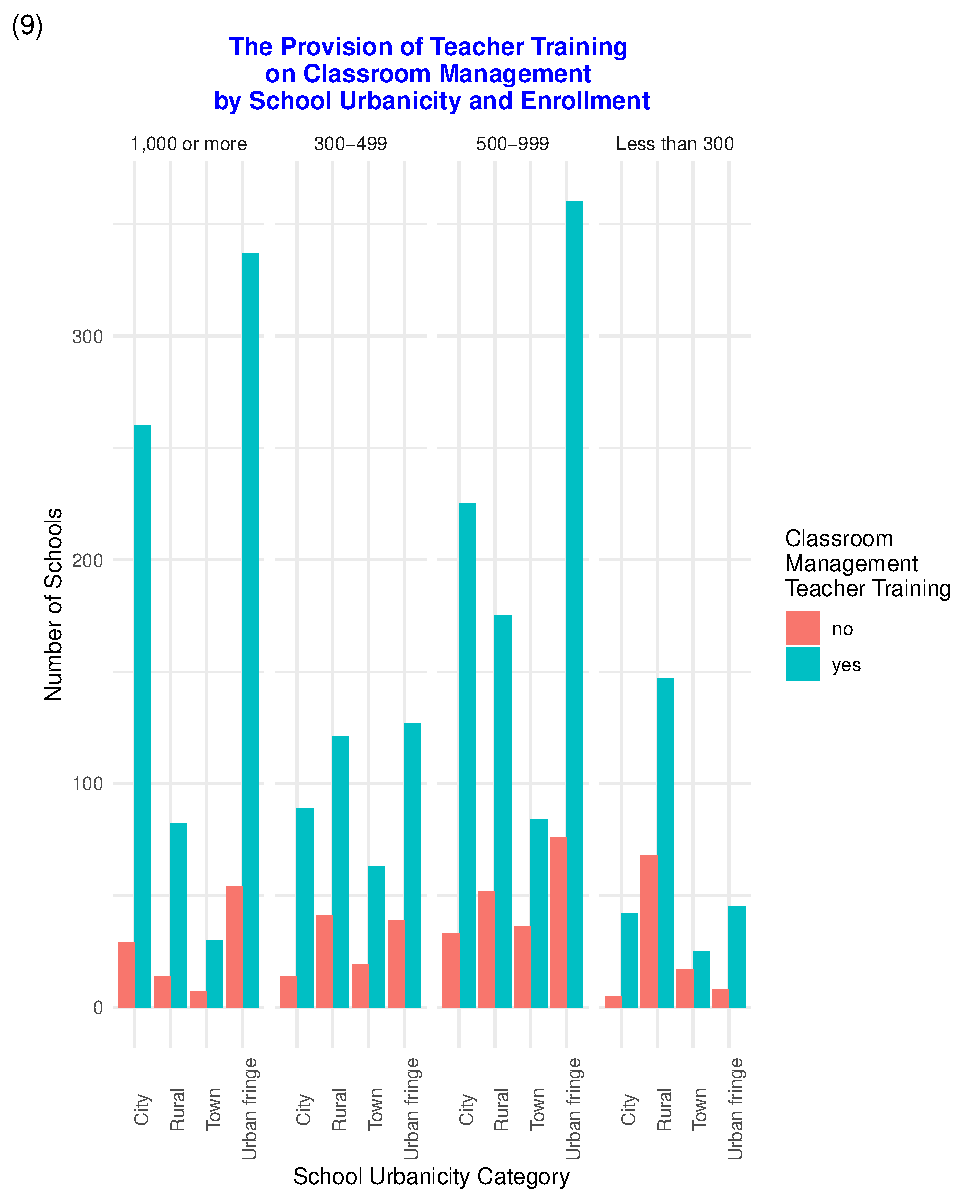
\includegraphics{Final-Project_Zhang_Wright_files/figure-latex/descriptives all selected data-4.pdf} 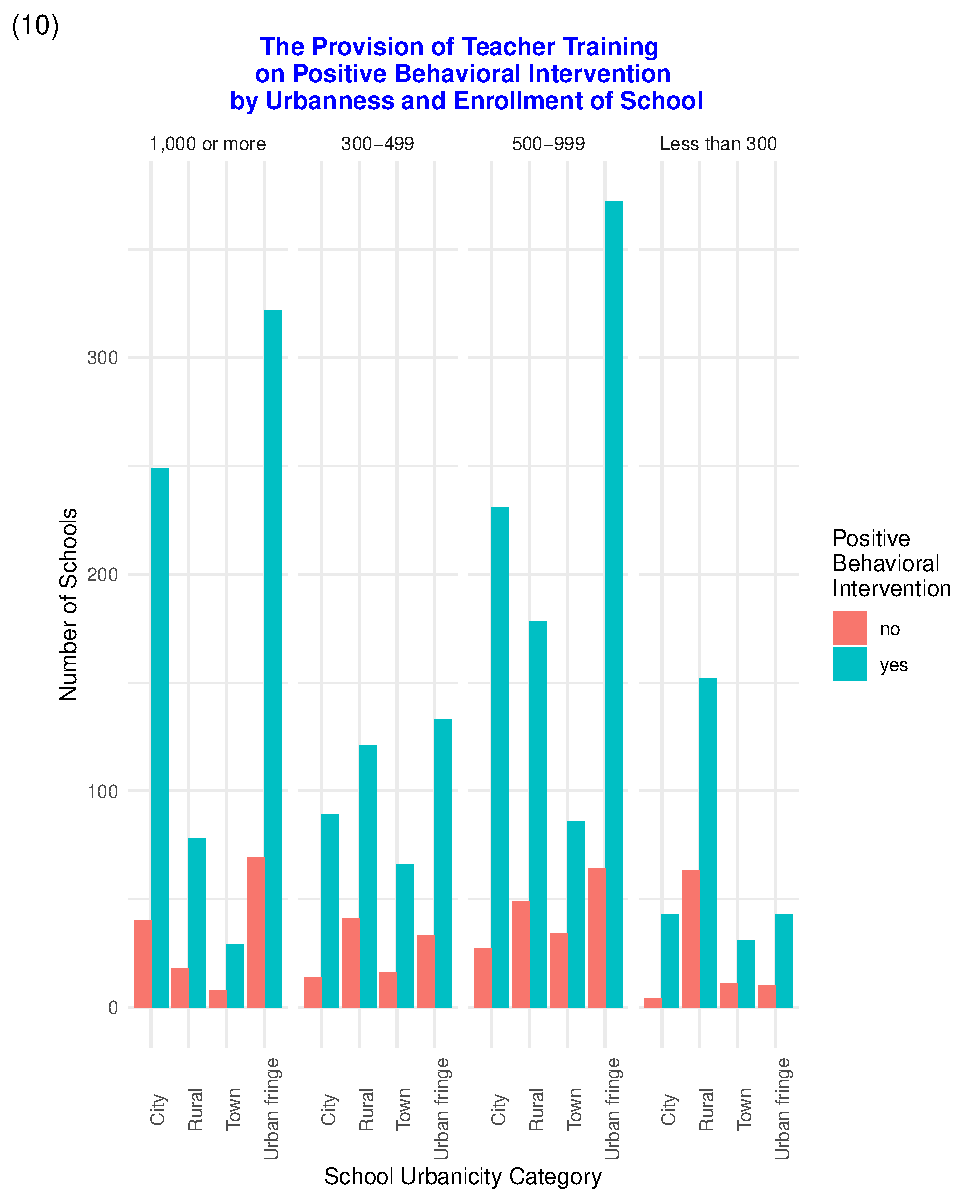
\includegraphics{Final-Project_Zhang_Wright_files/figure-latex/descriptives all selected data-5.pdf}

\begin{verbatim}
## Warning: Removed 160 rows containing non-finite values (stat_boxplot).
\end{verbatim}

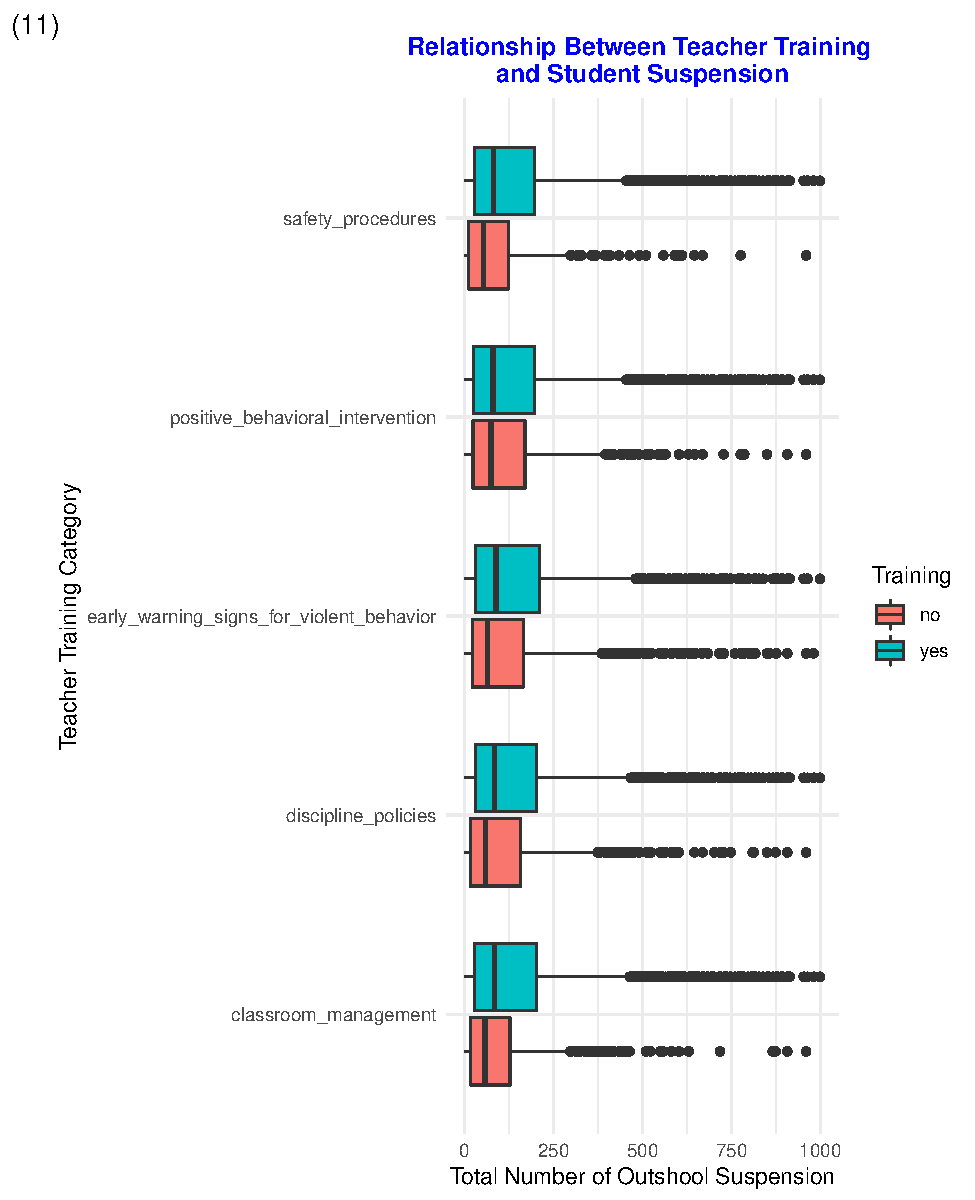
\includegraphics{Final-Project_Zhang_Wright_files/figure-latex/teacher training suspension visuals-1.pdf}

\begin{table}[tbp]
\begin{center}
\begin{threeparttable}
\caption{\label{tab:unnamed-chunk-1}Regression Results displaying Total Disciplinary Actions Predicted by Provision of Type of Teacher Training}
\begin{tabular}{ll}
\toprule
training & \multicolumn{1}{c}{total\_discipline\_actions}\\
\midrule
classroom\_management & 432,530.00\\
discipline\_policies & 432,530.00\\
early\_warning\_signs\_for\_violent\_behavior & 432,530.00\\
positive\_behavioral\_intervention & 432,530.00\\
safety\_procedures & 432,530.00\\
\bottomrule
\end{tabular}
\end{threeparttable}
\end{center}
\end{table}

\hypertarget{results}{%
\section{Results}\label{results}}

\hypertarget{tidy-data-1}{%
\subsection{Tidy data}\label{tidy-data-1}}

The mean number of total disciplinary actions was determined to be 159. This value was utilized to first identify schools with total disciplinary actions greater than this value and that did not provide any form of teacher training. A total of ten schools met the criteria. Five of these schools were coded for urbanicity as \emph{urban fringe}, two schools were coded as \emph{city}, two were coded as \emph{town}, and one school was coded as \emph{rural}. For the variable of school level, five of the schools were middle schools, four were high schools, and one school was a combined high school and middle school. For the variable of minority percentage, two schools possessed a minority percentage of \emph{50 percent or more}, four possessed a minority percentage of \emph{20 to 50 percent}, two possessed a minority percentage of \emph{5 to 20 percent}, and two schools possessed minority percentages of \emph{less than 5 percent}. Enrollment for four of the schools was coded as \emph{1,000 or more} students, \emph{500 - 999} students for three of the schools, \emph{300 - 499} for one of the schools, and \emph{less than 300} students for two of the schools.
Table 1 displays the descriptive statistics for the ten schools organized into the tidy data set. Plot 1 displays a bar graph with school urbanicity on the x-axis and the total number of disciplinary actions on the y-axis. Plot 2 is similar to plot 1 but has instead presented minority percentage on the x-axis and expanded the display of Plot 1 by adding the faceting the plot by school enrollment. The purpose of Plot 3 was to remove the facet() feature and reorder the levels of the minority percentage variable to appear in ascending order. Table 2 displays the descriptive statistics on the number of disciplinary actions per category of the ten schools filtered into the tidy data set. The use of the pivot\_wider() function allowed the data frame to return the four columns from the original data set: disciplinary actions recorded, incidents recorded, incidents reported to police, and out of school suspensions. Plots 4 and 5 provide exploratory scatterplots comparing the four variables of disciplinary actions. Plot 4 displays the total number of disciplinary actions recorded by the total number of incidents reported with a fill of minority percentage. Plot 5 displays the same comparison with a fill or urbanicity. It is the opinion of the authors that Plots 3 and 4 are not as useful as the other plots in terms of data visualization, but they did provide an extra opportunity to use features of ggplot, specifically the facet and fill functions.

\hypertarget{linear-models-1}{%
\subsection{Linear Models}\label{linear-models-1}}

Tables 3-5 display the results of the three linear models constructed to describe the total number of disciplinary actions taken by schools as predicted by school categorical variables.

\hypertarget{model-1}{%
\subsubsection{Model 1}\label{model-1}}

Model 1 was constructed to predict the total number of disciplinary actions by school urbanicity and school enrollment. This model accounted for approximately 20.05\% for the variance. The results of this model suggested that schools coded as \emph{city} with an enrollment of 1,000 or more students reported an average of 333.11 total disciplinary actions. Schools coded as \emph{rural} reported, on average, 52.18 fewer disciplinary actions when controlling for school enrollment. Additionally, schools coded as \emph{town} and \emph{urban fringe} reported an average of 34.26 and 39.84 fewer disciplinary actions when controlling for school enrollment. When controlling for school urbanicity, schools with enrollments of less than 1,000 students reported less disciplinary actions than schools with enrollments over 1,000. On average, schools with an enrollment of 300-499 students reported 231.59 less disciplinary actions, schools with an enrollment of 500-999 students reported 171.61 fewer disciplinary actions and schools with an enrollment of less than 300 reported 250.92 fewer disciplinary actions.

\hypertarget{model-2}{%
\subsubsection{Model 2}\label{model-2}}

Model 2 expanded upon Model 1 by adding a third predictor variable, school level. This model was determined to account for approximately 24.03\% of the variance. With the addition of the level variable, the results suggested that schools coded as \emph{city} and \emph{combined} with an enrollment of more than 1,000 students reported an average of 277.21 disciplinary actions. When controlling for urbanicity and enrollment, both high schools and middle schools reported larger numbers of disciplinary actions while primary schools reported fewer disciplinary actions. High schools reported an average of 76.29 more disciplinary actions and middle schools reported an average of 53.91 more disciplinary actions. Conversely, primary schools reported an average of 52.44 fewer disciplinary actions.

\hypertarget{model-3}{%
\subsubsection{Model 3}\label{model-3}}

Model 3 expanded upon Models 1 and 2 by adding the fourth categorical variable, minority percentage, as a predictor variable of total disciplinary actions. This model was determined to account for approximately 26.38\% of the variance. This model was determined to be the strongest model of predicting total disciplinary actions by school categorical variables. With the addition of the minority percentage variable, the results suggested that schools coded as \emph{city} and combined with an enrollment of more than 1,000 students and a minority percentage of 20-50\% reported an average of 249.19 total disciplinary actions. When controlling for urbanicity, enrollment, and level, schools in both the minority percentage categories of 5-20\% and less than 5\% reported fewer disciplinary actions. On average, schools with a minority percentage of 5-20\% reported 38.25\% fewer disciplinary actions while schools with a minority percentage of less than 5\% reported 32.42 fewer disciplinary actions. Conversely, schools with a minority percentage of 50\% or more reported a larger number of disciplinary actions compared to the 20-50\% category with an average of 48.62 more disciplinary actions.

\hypertarget{descriptive-data-exploration-and-visualization-1}{%
\subsection{Descriptive Data Exploration and Visualization}\label{descriptive-data-exploration-and-visualization-1}}

Plot 6 displays the 2,724 total schools included in the data set by their urbanicity and level categories. The most frequent urbanicity level was determined to be \emph{Urban fringe} with a total of 1,046 schools. Six hundred ninety-seven schools were coded as \emph{City}, 700 schools were coded as \emph{Rural}, and 281 schools were coded as \emph{Town}. The most frequent type of school included in the sample was middle schools with a total of 948 schools. The sample additionally consisted of 924 high schools, 715 primary schools, and 137 combined middle and high schools.

Plot 7 displays similar information to Plot 6 but with the additional aesthetic of faceting by school enrollment. The most frequent enrollment size included in the sample was determined to be \emph{500 - 999} students with a total of 1,041 schools. Eight hundred thirten schools reported an enrollment size of \emph{1,000 or more} students, 513 schools reported an enrollment of \emph{300 - 499} students, and 357 schools reported an enrollment size of \emph{less than 300} students.

Plot 8 displays a scatterplot to represent the relationship between the total number of out of school suspensions (oss) to the total number of disciplinary actions, a value that was created using the mutate() function to combine the total number of discipinary actions from the four quantitative variables included in the data set. There were determined to be 432,530 total disciplinary actions across all schools included in the data set, of which 42,199 were out of school suspensions (OSS). Overall, OSS accounted for 9.76\% of all disciplinary actions taken by schools.

\hypertarget{teacher-training-relationship-to-oss-1}{%
\subsection{Teacher Training Relationship to OSS}\label{teacher-training-relationship-to-oss-1}}

Plots 9 and 10 display descriptive counts on the number of schools that provide teacher training on classroom manageemnt and positive behaviorl intervention, respectively. Both plots are organized by school urbanicity and faceted by school enrollment. The purpose of Plot 11 was to visualize the relationship between five teacher training categories and the total number of OSS and help us to understand whether schools providing these teacher trainings or not have different OSS. From the plot we noticed that there are mean differences of OSS between training and no training in all categories except for positive behavioral intervention, but we don't know whether the differences are statistically significant or not. For positive behavioral training, the mean difference is fairly small which raises questions on whether this training is effective in reducing OSS. Overall, the relationship between teacher trainings and OSS is either unknown or unseen in this project, therefore further analysis is warranted if we want to know whether these five teacher trainings are effective ways to reduce OSS.

\hypertarget{discussion}{%
\section{Discussion}\label{discussion}}

The purpose of this project was to utilize the features and packages of R Markdown to perform data import, tidying, exploration, and visualization of the results of the 2005-2006 School Survey on Crime and Safety. Overall, the linear models and plots produced with R Markdown demonstrate results consistent with what has been previously established in the literature. Specifically, school disciplinary actions are most frequent in urban settings with large student enrollments and higher percentages of minority students. It is the opinion of the authors that more frequent and consistent provision of teacher training, specifically on positive behavior intervention, may be one method for schools to decrease their total number of disciplinary actions. Further investigation on the effect of teacher training on reducing total disciplinary actions is warranted.

The disparity in student discipline across such categorical variables as urbanicity, enrollment, and minority status aligns with concerns that has been previously identified in the literature (Han \& Akiba, 2011). Future studies should investigate the nature of discipline policy in more at risk schools to ensure specific groups of students are not over-targeted for disciplinary action.

\newpage

\hypertarget{references}{%
\section{References}\label{references}}

\begingroup
\setlength{\parindent}{-0.5in}
\setlength{\leftskip}{0.5in}

\hypertarget{refs}{}
\leavevmode\hypertarget{ref-chen2008}{}%
Chen, G. (2008). Communities, students, schools, and school crime: A confirmatory study of crime in us high schools. \emph{Urban Education}, \emph{43}(3), 301--318.

\leavevmode\hypertarget{ref-han2011}{}%
Han, S., \& Akiba, M. (2011). School safety, severe disciplinary actions, and school characteristics: A secondary analysis of the school survey on crime and safety. \emph{Journal of School Leadership}, \emph{21}(2), 262--292.

\leavevmode\hypertarget{ref-nolle2007}{}%
Nolle, K. L., Guerino, P., Dinkes, R., \& Chandler, K. (2007). Crime, violence, discipline, and safety in us public schools. Findings from the school survey on crime and safety: 2005-06. NCES 2007-361. \emph{National Center for Education Statistics}.

\endgroup

\end{document}
